\section{System Architecture}

% ---------------------------------------------------------------------------------------------------------------------
\subsection{Adapted version of the “Inner Thoughts” framework}
\label{sec:adapted-inner-thoughts}

\begin{figure}[H]
  \centering
  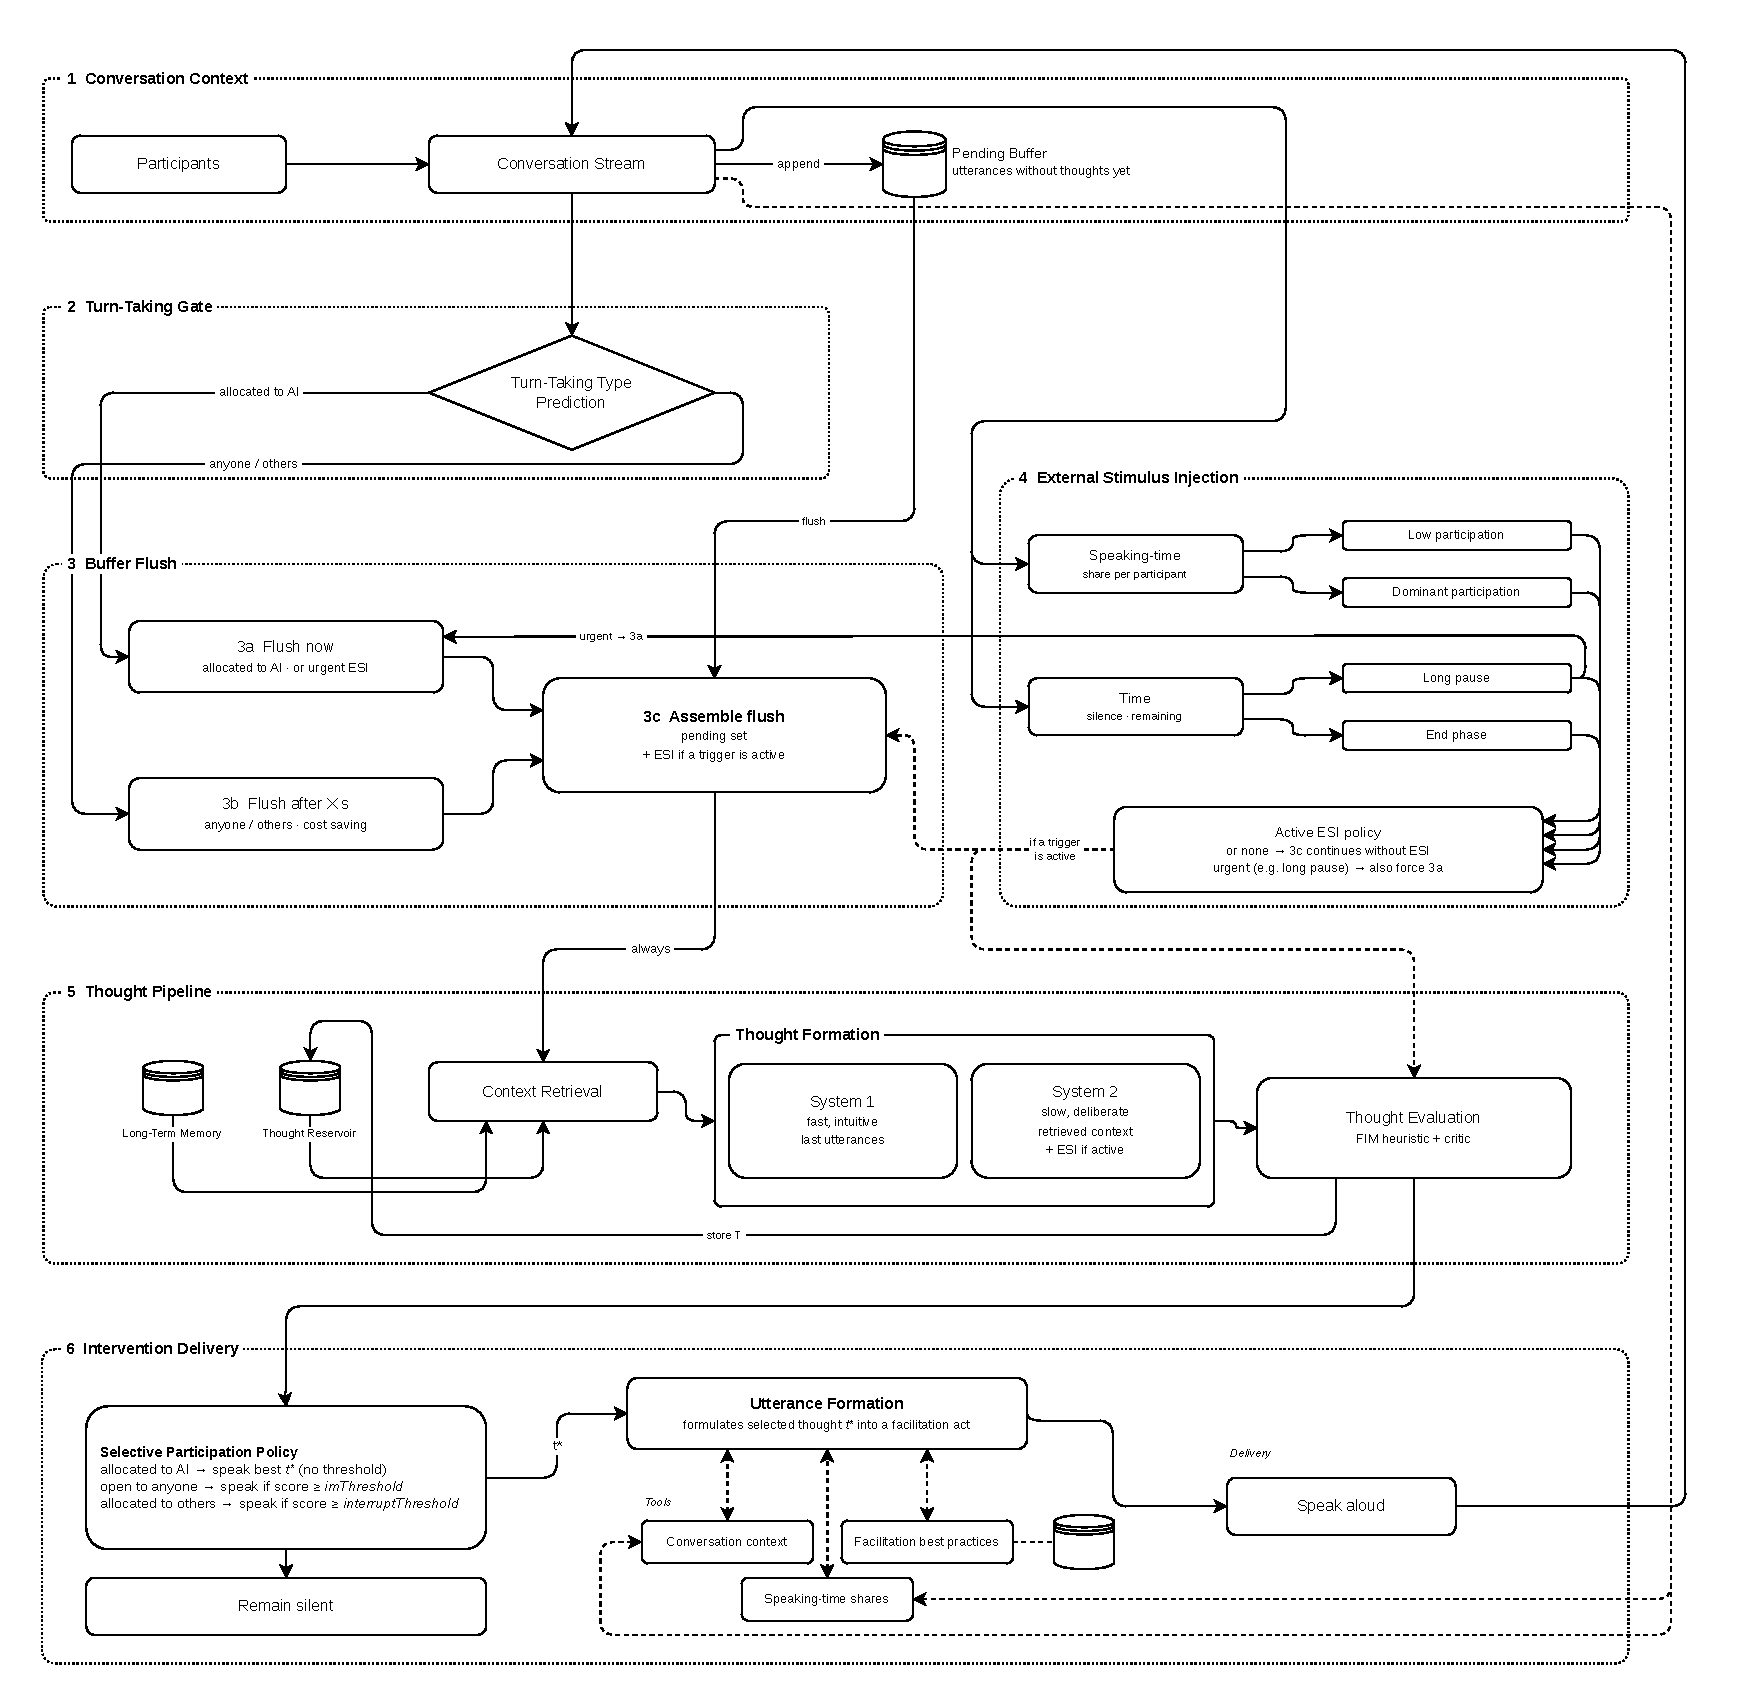
\includegraphics[width=0.99\textwidth]{assets/figures/04/system-architecture.pdf}
  \caption{System Architecture: Adapted version of the “Inner Thoughts” framework
    \figsource{Own illustration based on "Inner Thoughts" by Liu et
  al.\cite{liuProactiveConversationalAgents2025}, created with draw.io.}}
  \label{fig:system-architecture}
\end{figure}

\begin{figure}[H]
  \centering
  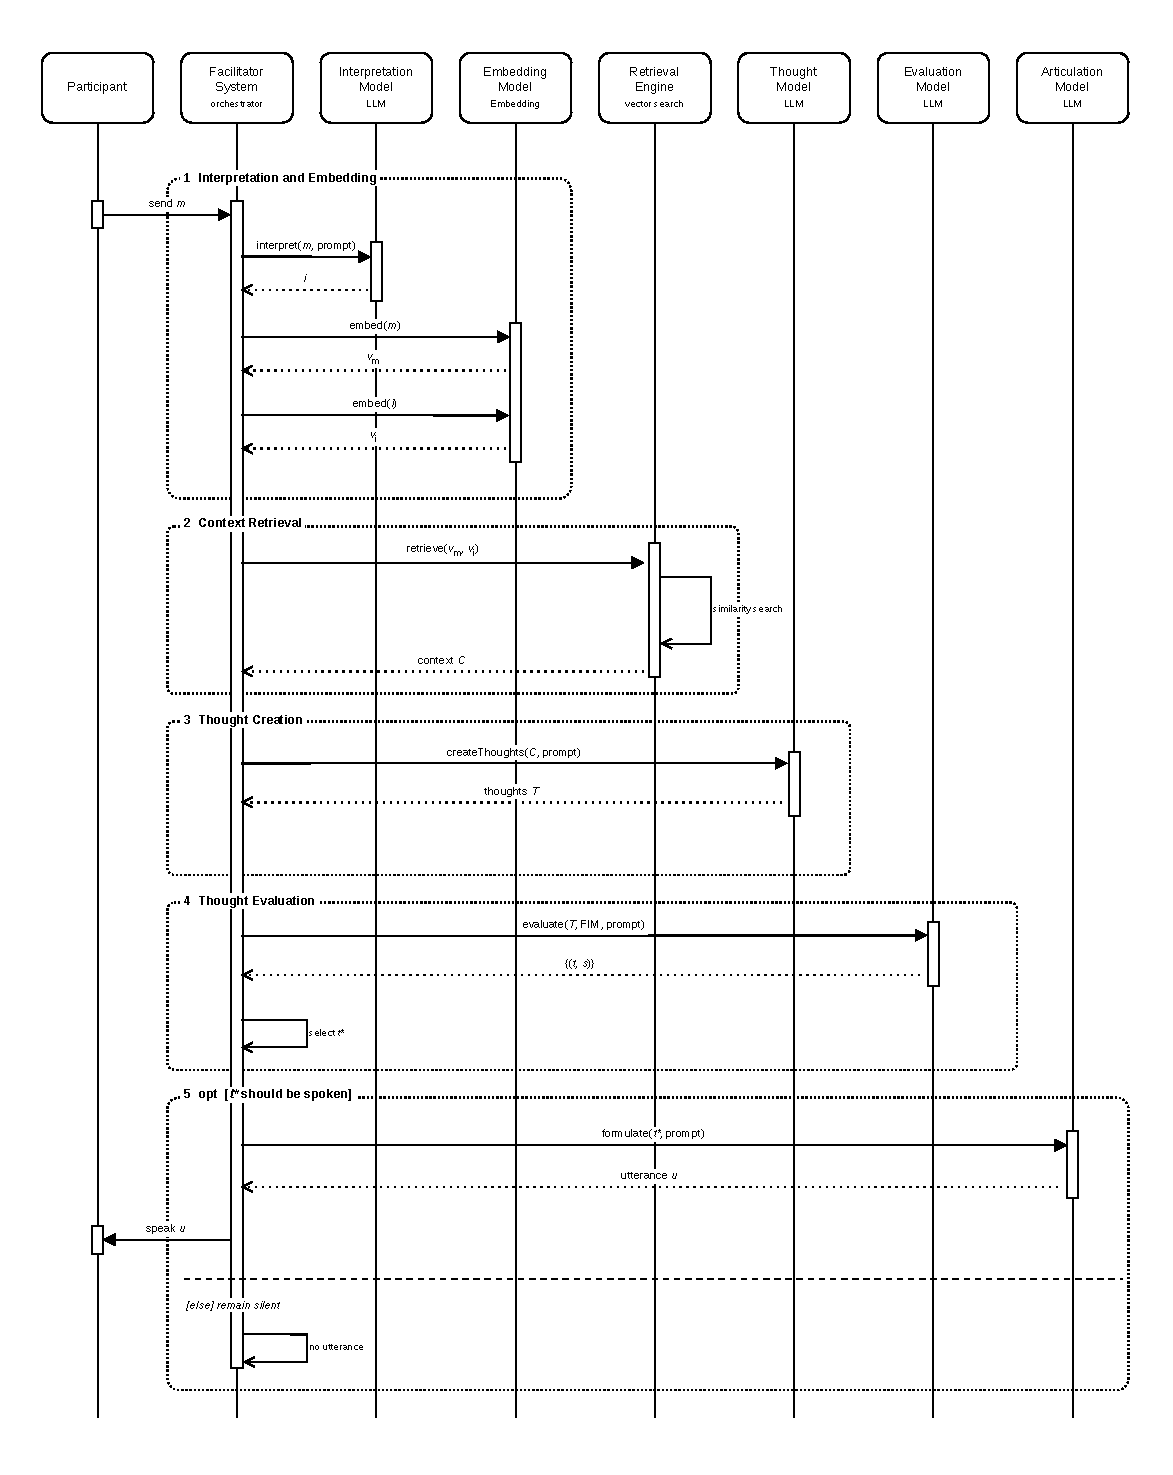
\includegraphics[width=0.97\textwidth]{assets/figures/04/thought-pipeline-sequence.pdf}
  \caption{Thought Pipeline Sequence: Sequence of the thought pipeline
    \figsource{Own illustration based on "Inner Thoughts" by Liu et
  al.\cite{liuProactiveConversationalAgents2025}, created with draw.io.}}
  \label{fig:thought-pipeline-sequence}
\end{figure}

Das Inner Thoughts- Freamwork von Liu et al. ist in deren version eher für interaktionen ausgelegt die als
soziales Plaudern kotegorisertet werden können. Dies ist nicht was ein Faciliator machen würde. Die Idee ein
KI-System anhand einer intrsisichen motivation zu modellieren, bevor jemand etwas zu einer Gruppen discussion
beiträgt, ist dennoch auch für diese ARbeit relevant.
Insbesondere weil dieser Ansatz darauf hindeutet eine erhöhte Genauigkeit bei self-trun-allocation zu erzeugen.
Aus den Experten ging hervor ds eine Geanken gänge, welche Facilitatoren haben auf abstakter inutionen
basieren andere wiederum druchdacht kombiniert mit experten wissen etc. Dies legt nach,
dass legt nahe das sowhl system 1 als auch system 2 bei dem prozess involoviert sind, was eben falls in dem
Innter Thougs Framewokr berücksichtigt wird.

Die Autoren wiesen in der Diskussion der Arbeit \cite["8.2 Apllying Inner Thougs Beyond Casual
Conversations"]{liuProactiveConversationalAgents2025} selbst darauf hin, dass sich das System durch anpassungen der
Bewertungskriterien auf aufgabenorietnerte Kontexte anpassen lässt und zielorientiertes praktives Handeln
ermöglichen kann. Sie schalgen vor für weitere arbieten das system mit domain-specifische heuristiken
anzupassen, um die interaktionen an real-world tasks zu orientieren.

Im ursprünglichen Modell von Liu et al. werden generierte Gedanken primär danach bewertet, wie stark sie die
"persönliche Relevanz" die individuellen Interessen oder die einzigartigen persönlichen Kenntnisse des
Agenten widerspiegeln (TODO: prüfen bzw. konkretisieren wie die heuristik tatsächlich ist). Dies mag für
generische Conversationen geeigent sein, da dieser Ansatz Authentizität und
Sympathie in infromellen, sozialen Unterhaltungen erhöht, ist für einen AI-Moderator in zielorientierne
Meetings die durch Hidden Profile geprägt sind, allerdings ungeeiengt. Wenn die Gedanken des AI-Moderator
primär danach bewertet würden, wie stark sie seinen "persönlichen Interssen" wiederspieglen, verfällt er in
dassaelber fehlerhafte Verahltensmuster, das zu verzeruung in hidden profile situationen führen kann. Er
bringt eingen Meinungen oder Präferzene ein statt die diskussion neutral zu strukturieren. Strukturelle
prozeduelle Gedanken würde in der aktuellen Heurisik voraussichtlich mit zu niederiger Relevanz bewertet werden.

Bei der Anpassung der Heurisitken und prompts wurden sowohl die Literatur als auch die erkentnisse aus den
Interviews berücksichtigt. Die Evaluierungs-Heursitik zu bewertung der Gedanken wurde so angepasst, dass sie
das kognitionspyschologsche Fundament des Innter Thoughts-Modelles (basierend  auf grice, Sacks, Goffman und
Berly) mit en organisationspsychologischen Prinzipien zur Kompenstation des Shared Information bias (Stasser \&
Titus; Brodbeck et al.) und den HCI-Richtlinen für inklusive Moderation (Houttie et al; Davison) kombiniert.

In der original Modellering des Inner Thougs-Frameworks wird ide participation in einer kovversation
ausschlielich basierend der innern gedanken abgeleitet. Die Authoern mekren an, dass exteren Cues nicht im
ausschleiieß zu ihrer Methode stehen sondern complentär mit exteren cues kombiniert zu einem robustern system
führen könnten. \cite[8.1 Proactive Agents via Intrinsic Motivation vs. Extrinsic
Cues]{liuProactiveConversationalAgents2025}

Eine kernproblematik bei hidden profies ist, das private inforamtione nicht getielt werden. Ein indikator
dafür könnte sein, dass eine person sich an der converstation nicht beteiligt oder ander Teilnehmden die
Diskussion domieren, so dass andere nicht zu wort kommen können. wie aus den interviews
hervorging, würde ein facilitator hier typischer weise versuchen diese Person auf höfliche art zu integrieen,
um deren Perspektive zu hören. Hierfür wäre extern Cues wie die Sprrecheranteile relevant. Um diese
exteren Cues abzubilden wurde das Inner Thoughs Framework, um die Komponete "External Stimulus Injection" erweitert.
Ist einer dieser externe Trigger erfüllt wird ein vordefinierter Gedanke in der Gedanken generierung von
System 2 berügcksichtig und die Evaluations herusitik bewsust in richtung diesen extern Triggers gebaiased,
um zu erzielen dass diese externe cue im innerthoughs modeel gewichtet wird.

%%%%%%%%%
Baseirend auf der Literatur und den Intervies wurde versucht dieses System entpsrechend zu adaptieren.

Ein prblem ist die tendenz von KI zu überkompensieren und zu viel zu sagen. Die authoren merken dies auch an
und sind optimistischen, dasss ihr conversational agent hier besser performt. Alelrdigns handelt es sich um
eine plausch. Ein facilitator würde nicht so oft in die Diskussion eingreifen. Das risiko für
overcompensationg mit diesem system ist hoch. mit dem imThreshold kann gesteuert werden wie schwerwwiegend
ein Gedanke sein muss damit die KI ihn überhaupt aussproche.

In dem Paper wurd ein Selective Participant modeliert, welche foglende Parameter hatte:

- System1 wurde auf 0 gesetzt so das die KI also niemals äußert niemals spontane, ungeplante
System-1-Floskeln äußert. Jeder Beitrag muss einen teifen, kognitiven Nutzen haben.
-imThreshold wurde auf 4.3 gesetzt. Ein strategeischer Gedanke muss auf einer Skala von 1-5 einen extrem
hohe Bewertung erreichen, um die schwelle zu reißen. Ein einfacher Gedanke wie "ICh könnte Bob mal wieder
fragen" reicht dafür nicht aus. Es bedarf eines
Phase 1 Trigger:

% ---------------------------------------------------------------------------------------------------------------------
\subsection{Components: Transcription, Analysis, and Intervention Modules}

Abgleeite aus dem Paper Keeper. Der Agent könnte auch eine visualle Warteschlage steuern. anstatt aktiv zu
unterbrechen sezt ersich auf die warteschalge bzw. hebt die hand, um sich anzukündigen.
% Wenn dein AI-Facilitator interveniert, um den Shared Information Bias zu brechen, muss er dies nicht zwingend
% über eine störende, verbale Unterbrechung tun. Du kannst vorschlagen, dass der Agent eine visuelle
% Warteschlange steuert (z. B. "Ich setze Bob als nächsten auf die Rednerliste, da er zu Kriterium X wertvolle
% ungeteilte Infos hat"). Das senkt die kognitive Last der Teilnehmer und sichert ihre Aufmerksamkeit.

\textbf{FIM-Heuristik}

\textbf{Thought-Evaluation}

The full FIM scoring prompt, with a unit-by-unit provenance relative to the
original Inner Thoughts evaluation protocol, is documented in
\autoref{annex:fim-scoring}.

Angelengt an die Thoguht Evaluation Phase von XX (procativ Conversation Agents) wurde auch in diesem sich dem
contextual self-refinement bedient.
Self-Refinement und Reflexion könnnen bei LLMs zu drastischen ELsitugssteirgunen führen, wenn eine kognitive
Feedbackschleife druchaufen wird. \cite[p. 18]{meiSurveyContextEngineering2025} Ein Gedanke wird nicht direkt
ausgesprochen, sondern druch einen Kritiker basierend auf der für diese arbeit entwicklete FIM-Heurisitk geprüft.
The evaluation protocol follows the G-Eval prompt structure \cite[p. 2512]{liuGEvalNLGEvaluation2023}
similarly also used for Thoughtful Agents. Probability-weighted scoring as proposed in the original method
was omitted as a pragmatic decision, because the APIs used here do not return output-token probabilities.

In practice every utterance is appended to a shared pending buffer of messages that have not yet
been thought about. The turn-taking prediction only decides \emph{when} that buffer is flushed
(immediately if the floor is allocated to the AI; otherwise after $X$ seconds as one batch). Both
cases continue to the same next step: the flushed pending set is assembled and the thought pipeline
runs. External Stimulus Injection is not a later stage. Its monitors run continuously, but an ESI
policy joins the pipeline only at that flush, and only if a trigger is active; otherwise the
pipeline runs without it. A selected thought $t^{*}$ is not spoken raw. An Utterance Formation
agent formulates it into a facilitation act, with tools for conversation context, facilitation best
practices, speaking-time shares, sending a chat message, or speaking aloud.
The articulation prompt and the mapping from the original Inner Thoughts
wording are documented in \autoref{annex:articulation-prompt}.

\autoref{tab:architecture-design-decisions} maps each architectural choice to a single warrant and to the
chapters that already establish it, so the implementation can be traced without restating those arguments.
\clearpage
\begin{table}[H]
  \centering
  \caption{Architectural design decisions of the adapted Inner Thoughts prototype, with rationale and
  pointers to the motivating chapters of this thesis.}
  \label{tab:architecture-design-decisions}
  \small
  \setlength{\tabcolsep}{4pt}
  \begin{tabularx}{\textwidth}{@{}
      >{\raggedright\arraybackslash}p{2.85cm}
      >{\raggedright\arraybackslash}X
      >{\raggedright\arraybackslash}p{3.55cm}
    @{}}
    \toprule
    \textbf{Design decision} & \textbf{Rationale} & \textbf{Evidence} \\
    \midrule
    Adapt Inner Thoughts from casual talk to facilitation
    & The original model times utterances by intrinsic motivation, which improves self-turn-allocation
    in multi-party talk. Liu et~al.\ already invite domain-specific evaluation criteria for
    goal-directed settings; without that shift, a facilitator would be scored as a social
    conversationalist.
    & \autoref{sec:proactive-ai-interactions} \\
    \addlinespace
    Replace personal-relevance scoring with a facilitation-oriented FIM heuristic
    & Ranking thoughts by the agent's own interests would privilege preference talk, undervalue
    procedural structure, and reproduce the shared-information bias the moderator is meant to
    counteract.
    & \autoref{sec:hidden-profiles};
    \autoref{ch:empirical-analysis-of-facilitating-strategies} \\
    \addlinespace
    Inject external participation cues into thought generation
    & Unique information stays private when speakers remain silent or are crowded out. Observable
    speaking-time imbalance is a complementary cue, not a rival, to intrinsic motivation; expert
    facilitators report inviting quiet members rather than waiting for self-selection.
    & \autoref{sec:hidden-profiles};
    \autoref{sec:key-challenges-in-meetings};
    \autoref{ch:empirical-analysis-of-facilitating-strategies} \\
    \addlinespace
    Selective-participant policy: no System-1 speech, high \textit{imThreshold}
    & Facilitation needs sparse, high-utility interventions. Unconstrained generation over-talks;
    disabling System-1 filler and raising the utterance threshold admits only thoughts with clear
    process value.
    & \autoref{sec:facilitation};
    \autoref{sec:interaction-paradigms} \\
    \addlinespace
    Critic-based self-refinement before any utterance
    & A thought is spoken only after a critic applies the FIM heuristic. Contextual self-refinement
    implements an evaluator--optimizer loop and is associated with substantial quality gains in
    LLM pipelines.
    & \autoref{sec:context-engineering};
    \autoref{sec:ai-agent-building-blocks} \\
    \addlinespace
    Cheap temporal reweighting instead of LLM re-scoring
    & Static IM speaks stale thoughts. Re-prompting every thought after each event is too slow and
    costly for a live meeting. Linear aging and a post-speech smoothstep keep the original score
    but discount age and repetition.
    & \autoref{sec:adapted-inner-thoughts} \\
    \bottomrule
  \end{tabularx}
\end{table}
\FloatBarrier

\minisec{Dynamic intrinsic motivation}
\label{sec:dynamic-im}

In the original Inner Thoughts model, intrinsic motivation is static: a thought is scored once at
generation and that score never changes. Early tests showed the consequence: the agent spoke thoughts
that the subsequent discussion had already made obsolete, and that would no longer have received a
high FIM score given how the meeting had evolved.

% TODO: beispielhafter Chatverlauf, in dem ein statischer FIM-Score zu spät geäußert wird.

Re-scoring every pending thought with an LLM after each event would restore recency, but the added
latency and cost would make the system unusable in a live meeting. The prototype therefore keeps the
original FIM score and applies a cheap, deterministic reweighting under two assumptions.
\begin{itemize}
  \item A thought becomes a poorer description of the current state as the conversation moves on, because later
    information was not available when it was scored; its priority should fall with age.
  \item Once a thought has been spoken, the motivation to say it again is initially very low, but may recover if the
    group does not take it up.
\end{itemize}
These two effects address different failure modes, so they multiply.
With \(s_0\) the base FIM score, \(t\) the age in seconds, and \(c\) a cooldown factor,

\begin{equation}
  s_{\mathrm{aged}}(t)
  =\max\bigl(0,\, s_0(1-t/H)\bigr),
  \qquad
  s_{\mathrm{eff}}
  =\min\bigl(5,\, \max(0,\, s_{\mathrm{aged}}\cdot c)\bigr).
  \label{eq:im-aged-eff}
\end{equation}

\paragraph{Why linear.}
A linear kernel is the simplest decay that hits zero in finite time and can be inverted from an
operational requirement: choose how long a thought of score \(s_{\mathrm{hold}}\) must stay above
\(\tau\). That fixes the slope. An exponential never reaches zero, so a residual could later
interact with cooldown recovery. A downward parabola with a flat start would delay the first loss of
score, then drop faster; that grace period is a modelling preference, not a property measured in the
meetings. Linear already lets weaker thoughts expire sooner, because they start closer to \(\tau\)
(\autoref{fig:im-aging}).

\paragraph{Why this horizon.}
\(H\) is not a fitted half-life. It is inverted from an operational requirement: a thought with score
\(s_{\mathrm{hold}}\) must remain above \(\tau\) for exactly \(t_{\mathrm{hold}}\) seconds.
Substituting \(s_{\mathrm{aged}}(t_{\mathrm{hold}})=\tau\) yields

\begin{equation}
  H=\frac{t_{\mathrm{hold}}}{1-\tau/s_{\mathrm{hold}}}.
  \label{eq:im-horizon}
\end{equation}

All thoughts share this \(H\). A weaker thought, already closer to \(\tau\), therefore drops below
the threshold sooner than a stronger one. The pair \((s_{\mathrm{hold}}, t_{\mathrm{hold}})\) is the
only design knob for temporal sensitivity. Read left to right in
\autoref{fig:im-aging}: a shorter \(t_{\mathrm{hold}}\) steepens every line and pulls
every crossing to the left, including weaker thoughts.

\begin{figure}[H]
  \centering
  % Linear FIM aging: effect of t_hold. Small multiples for t_hold in {20, 45, 90} s.
% Shared standalone preamble for the dynamic-FIM PGFPlots figures.
% Compiled from the repository root via scripts/build-tikz-figures.sh.
\documentclass[11pt,border=0pt]{standalone}
\usepackage{pgfplots}
\pgfplotsset{compat=1.18}
\tikzset{hide legend/.code={}}
\usepackage[accentcolor=TUDa-2c]{tudacolors}
\usepackage{tudafonts}

% Match the thesis typearea \textwidth so 0.32\textwidth panels stay the same.
\newlength{\imfigwidth}
\setlength{\imfigwidth}{418.25555pt}

% Shared pgfplots styles and IM kernels for the dynamic-FIM figures.
% Illustrative calibration: tau=4.3, s_hold=5, t_hold=45 s, t_cool=60 s, spoken at 12 s.
\ifdefined\IMdynamicsStylesLoaded\else
\newcommand{\IMdynamicsStylesLoaded}{}
\pgfplotsset{
  IM functions/.style={
    declare function={
      tau=4.3;
      shold=5.0;
      thold=45.0;
      tcool=60.0;
      tspk=12.0;
      Hor=thold/(1-tau/shold);
      aged(\s,\t)=max(0,\s*(1-\t/Hor));
      agedH(\s,\t,\th)=max(0,\s*(1-\t*(1-tau/shold)/\th));
      smstep(\x)=ifthenelse(\x<0,0,ifthenelse(\x>1,1,3*\x*\x-2*\x*\x*\x));
      cool(\ts)=smstep(\ts/tcool);
      coolH(\ts,\tc)=smstep(\ts/\tc);
      linH(\ts,\tc)=min(1,\ts/\tc);
      spoken(\t)=aged(5,\t)*ifthenelse(\t<tspk,1,cool(\t-tspk));
    }
  },
  IMcore/.style={
    IM functions,
    font=\footnotesize,
    tick label style={font=\scriptsize},
    label style={font=\footnotesize},
    title style={font=\footnotesize, at={(0.0,1.0)}, anchor=south west, yshift=4pt},
    axis lines=left,
    axis line style={{}-{}},
    tick align=outside,
    clip=true,
    grid=major,
    grid style={TUDa-0a, thin},
    every axis plot/.append style={line cap=round, line join=round},
  },
  IMaxis/.style={
    IMcore,
    legend cell align=left,
    legend style={
      font=\scriptsize,
      draw=none,
      fill=none,
      inner sep=1.5pt,
      row sep=-0.5pt,
      cells={anchor=west},
    },
  },
  IMhold/.style={
    IMcore,
    width=\linewidth,
    height=4.45cm,
    xlabel={Age $t$ (s)},
    xmin=0, xmax=100,
    ymin=0, ymax=5.55,
    xtick={0,20,40,60,80,100},
    extra y ticks={4.3},
    extra y tick labels={$\tau$},
    extra y tick style={grid=none, tick label style={font=\scriptsize}},
    domain=0:100,
    samples=80,
  },
  IMcool/.style={
    IMcore,
    width=\linewidth,
    height=4.45cm,
    xlabel={Seconds since spoken $t_{\mathrm{spk}}$},
    xmin=0, xmax=120,
    ymin=0, ymax=1.15,
    xtick={0,30,60,90,120},
    ytick={0,0.25,0.5,0.75,1},
    domain=0:120,
    samples=100,
  },
}
\fi



\begin{document}
\begin{minipage}{\imfigwidth}
\noindent
\begin{minipage}[t]{0.32\textwidth}
  \centering
  \begin{tikzpicture}
    \begin{axis}[
        IMhold,
        title={$t_{\mathrm{hold}}{=}20\,\mathrm{s}$},
        ylabel={Aged score $s_{\mathrm{aged}}$},
      ]
      \addplot[TUDa-8b, solid, very thick] {agedH(4.5,x,20)};
      \addplot[TUDa-3b, solid, very thick] {agedH(4.7,x,20)};
      \addplot[TUDa-1b, solid, very thick] {agedH(5,x,20)};
      \addplot[TUDa-9b, dashdotted, thick, domain=0:100, samples=2] {tau};
      \addplot[TUDa-8b, only marks, mark=*, mark size=1.5pt]
      coordinates {(6.35,4.3)};
      \addplot[TUDa-3b, only marks, mark=*, mark size=1.5pt]
      coordinates {(12.16,4.3)};
      \addplot[TUDa-1b, only marks, mark=*, mark size=1.5pt]
      coordinates {(20.00,4.3)};
      \addplot[TUDa-0d, dashed] coordinates {(20,0) (20,5.15)}
      node[pos=0.24, anchor=west, font=\scriptsize, inner sep=1.5pt, black]
      {$t_{\mathrm{hold}}$};
    \end{axis}
  \end{tikzpicture}
\end{minipage}%
\hfill
\begin{minipage}[t]{0.32\textwidth}
  \centering
  \begin{tikzpicture}
    \begin{axis}[
        IMhold,
        title={$t_{\mathrm{hold}}{=}45\,\mathrm{s}$},
        ylabel={},
        yticklabels={},
      ]
      \addplot[TUDa-8b, solid, very thick] {agedH(4.5,x,45)};
      \addplot[TUDa-3b, solid, very thick] {agedH(4.7,x,45)};
      \addplot[TUDa-1b, solid, very thick] {agedH(5,x,45)};
      \addplot[TUDa-9b, dashdotted, thick, domain=0:100, samples=2] {tau};
      \addplot[TUDa-8b, only marks, mark=*, mark size=1.5pt]
      coordinates {(14.29,4.3)};
      \addplot[TUDa-3b, only marks, mark=*, mark size=1.5pt]
      coordinates {(27.36,4.3)};
      \addplot[TUDa-1b, only marks, mark=*, mark size=1.5pt]
      coordinates {(45.00,4.3)};
      \addplot[TUDa-0d, dashed] coordinates {(45,0) (45,5.15)}
      node[pos=0.24, anchor=west, font=\scriptsize, inner sep=1.5pt, black]
      {$t_{\mathrm{hold}}$};
    \end{axis}
  \end{tikzpicture}
\end{minipage}%
\hfill
\begin{minipage}[t]{0.32\textwidth}
  \centering
  \begin{tikzpicture}
    \begin{axis}[
        IMhold,
        title={$t_{\mathrm{hold}}{=}90\,\mathrm{s}$},
        ylabel={},
        yticklabels={},
      ]
      \addplot[TUDa-8b, solid, very thick] {agedH(4.5,x,90)};
      \addplot[TUDa-3b, solid, very thick] {agedH(4.7,x,90)};
      \addplot[TUDa-1b, solid, very thick] {agedH(5,x,90)};
      \addplot[TUDa-9b, dashdotted, thick, domain=0:100, samples=2] {tau};
      \addplot[TUDa-8b, only marks, mark=*, mark size=1.5pt]
      coordinates {(28.57,4.3)};
      \addplot[TUDa-3b, only marks, mark=*, mark size=1.5pt]
      coordinates {(54.71,4.3)};
      \addplot[TUDa-1b, only marks, mark=*, mark size=1.5pt]
      coordinates {(90.00,4.3)};
      \addplot[TUDa-0d, dashed] coordinates {(90,0) (90,5.15)}
      node[pos=0.24, anchor=east, font=\scriptsize, inner sep=1.5pt, black]
      {$t_{\mathrm{hold}}$};
    \end{axis}
  \end{tikzpicture}
\end{minipage}

\vspace{0.2em}
{\centering
  \scriptsize
  \begin{tikzpicture}[baseline=-0.4ex]
    \draw[TUDa-8b, very thick] (0,0) -- (0.55,0);
  \end{tikzpicture}~$s_0{=}4.5$
  \hspace{0.9em}
  \begin{tikzpicture}[baseline=-0.4ex]
    \draw[TUDa-3b, very thick] (0,0) -- (0.55,0);
  \end{tikzpicture}~$s_0{=}4.7$
  \hspace{0.9em}
  \begin{tikzpicture}[baseline=-0.4ex]
    \draw[TUDa-1b, very thick] (0,0) -- (0.55,0);
  \end{tikzpicture}~$s_0{=}5.0$
  \hspace{0.9em}
  \begin{tikzpicture}[baseline=-0.4ex]
    \draw[TUDa-9b, dashdotted, thick] (0,0) -- (0.55,0);
  \end{tikzpicture}~$\tau{=}4.3$\par
}
\end{minipage}
\end{document}

  \caption{Linear aging of the FIM score at three hold-times. Each panel shows the same
    scores \(s_0\in\{4.5,4.7,5.0\}\); the vertical line is \(t_{\mathrm{hold}}\), where a
    score-5 thought crosses \(\tau\). Within a panel, weaker thoughts expire sooner. Left to
    right, a shorter \(t_{\mathrm{hold}}\) steepens every line.
    Parameters: \(\tau=4.3\), \(s_{\mathrm{hold}}=5\).
  \figsource{Own illustration.}}
  \label{fig:im-aging}
\end{figure}

\paragraph{Why a smoothstep after speech.}
If a thought has never been spoken, \(c=1\). After it has been spoken, with \(t_{\mathrm{spk}}\) the
seconds since articulation and \(t_{\mathrm{cool}}\) the recovery window,

\begin{equation}
  c=\mathrm{smoothstep}(t_{\mathrm{spk}}/t_{\mathrm{cool}}),
  \qquad
  \mathrm{smoothstep}(x)=
  \begin{cases}
    0 & x\le 0,\\
    3x^{2}-2x^{3} & 0<x<1,\\
    1 & x\ge 1.
  \end{cases}
  \label{eq:im-smoothstep}
\end{equation}

The cubic \(3x^{2}-2x^{3}\) is the Hermite interpolant that is 0 at 0 and 1 at 1, with zero
derivative at both ends. A linear ramp would start climbing immediately---the same facilitation move
could reappear within seconds---and would kink at \(t_{\mathrm{cool}}\)
(\autoref{fig:im-cooldown}). The flat start enforces a true pause; the flat end hands control back
to aging without a jump in slope. The prototype uses \(t_{\mathrm{cool}}=60\,\mathrm{s}\);
shorter and longer windows stretch the same shape.

\begin{figure}[H]
  \centering
  % Cooldown factor after speech. Small multiples for t_cool in {30, 60, 90} s.
% Shared pgfplots styles and IM kernels for the dynamic-FIM figures.
% Illustrative calibration: tau=4.3, s_hold=5, t_hold=45 s, t_cool=60 s, spoken at 12 s.
\ifdefined\IMdynamicsStylesLoaded\else
\newcommand{\IMdynamicsStylesLoaded}{}
\pgfplotsset{
  IM functions/.style={
    declare function={
      tau=4.3;
      shold=5.0;
      thold=45.0;
      tcool=60.0;
      tspk=12.0;
      Hor=thold/(1-tau/shold);
      aged(\s,\t)=max(0,\s*(1-\t/Hor));
      agedH(\s,\t,\th)=max(0,\s*(1-\t*(1-tau/shold)/\th));
      smstep(\x)=ifthenelse(\x<0,0,ifthenelse(\x>1,1,3*\x*\x-2*\x*\x*\x));
      cool(\ts)=smstep(\ts/tcool);
      coolH(\ts,\tc)=smstep(\ts/\tc);
      linH(\ts,\tc)=min(1,\ts/\tc);
      spoken(\t)=aged(5,\t)*ifthenelse(\t<tspk,1,cool(\t-tspk));
    }
  },
  IMcore/.style={
    IM functions,
    font=\footnotesize,
    tick label style={font=\scriptsize},
    label style={font=\footnotesize},
    title style={font=\footnotesize, at={(0.0,1.0)}, anchor=south west, yshift=4pt},
    axis lines=left,
    axis line style={{}-{}},
    tick align=outside,
    clip=true,
    grid=major,
    grid style={TUDa-0a, thin},
    every axis plot/.append style={line cap=round, line join=round},
  },
  IMaxis/.style={
    IMcore,
    legend cell align=left,
    legend style={
      font=\scriptsize,
      draw=none,
      fill=none,
      inner sep=1.5pt,
      row sep=-0.5pt,
      cells={anchor=west},
    },
  },
  IMhold/.style={
    IMcore,
    width=\linewidth,
    height=4.45cm,
    xlabel={Age $t$ (s)},
    xmin=0, xmax=100,
    ymin=0, ymax=5.55,
    xtick={0,20,40,60,80,100},
    extra y ticks={4.3},
    extra y tick labels={$\tau$},
    extra y tick style={grid=none, tick label style={font=\scriptsize}},
    domain=0:100,
    samples=80,
  },
  IMcool/.style={
    IMcore,
    width=\linewidth,
    height=4.45cm,
    xlabel={Seconds since spoken $t_{\mathrm{spk}}$},
    xmin=0, xmax=120,
    ymin=0, ymax=1.15,
    xtick={0,30,60,90,120},
    ytick={0,0.25,0.5,0.75,1},
    domain=0:120,
    samples=100,
  },
}
\fi


\noindent
\begin{minipage}[t]{0.32\textwidth}
  \centering
  \begin{tikzpicture}
    \begin{axis}[
        IMcool,
        title={$t_{\mathrm{cool}}{=}30\,\mathrm{s}$},
        ylabel={Cool factor $c$},
      ]
      \addplot[TUDa-0c, densely dashed, thick] {linH(x,30)};
      \addplot[TUDa-1b, solid, very thick] {coolH(x,30)};
      \addplot[TUDa-0d, dashed] coordinates {(30,0) (30,1.05)}
      node[pos=0.22, anchor=west, font=\scriptsize, inner sep=1.5pt, black]
      {$t_{\mathrm{cool}}$};
    \end{axis}
  \end{tikzpicture}
\end{minipage}%
\hfill
\begin{minipage}[t]{0.32\textwidth}
  \centering
  \begin{tikzpicture}
    \begin{axis}[
        IMcool,
        title={$t_{\mathrm{cool}}{=}60\,\mathrm{s}$},
        ylabel={},
        yticklabels={},
      ]
      \addplot[TUDa-0c, densely dashed, thick] {linH(x,60)};
      \addplot[TUDa-1b, solid, very thick] {coolH(x,60)};
      \addplot[TUDa-0d, dashed] coordinates {(60,0) (60,1.05)}
      node[pos=0.22, anchor=west, font=\scriptsize, inner sep=1.5pt, black]
      {$t_{\mathrm{cool}}$};
    \end{axis}
  \end{tikzpicture}
\end{minipage}%
\hfill
\begin{minipage}[t]{0.32\textwidth}
  \centering
  \begin{tikzpicture}
    \begin{axis}[
        IMcool,
        title={$t_{\mathrm{cool}}{=}90\,\mathrm{s}$},
        ylabel={},
        yticklabels={},
      ]
      \addplot[TUDa-0c, densely dashed, thick] {linH(x,90)};
      \addplot[TUDa-1b, solid, very thick] {coolH(x,90)};
      \addplot[TUDa-0d, dashed] coordinates {(90,0) (90,1.05)}
      node[pos=0.22, anchor=east, font=\scriptsize, inner sep=1.5pt, black]
      {$t_{\mathrm{cool}}$};
    \end{axis}
  \end{tikzpicture}
\end{minipage}

\vspace{0.2em}
{\centering
  \scriptsize
  \begin{tikzpicture}[baseline=-0.4ex]
    \draw[TUDa-0c, densely dashed, thick] (0,0) -- (0.55,0);
  \end{tikzpicture}~linear ramp
  \hspace{0.9em}
  \begin{tikzpicture}[baseline=-0.4ex]
    \draw[TUDa-1b, very thick] (0,0) -- (0.55,0);
  \end{tikzpicture}~smoothstep
  \hspace{0.9em}
  \begin{tikzpicture}[baseline=-0.4ex]
    \draw[TUDa-0d, dashed] (0,0) -- (0.55,0);
  \end{tikzpicture}~$t_{\mathrm{cool}}$\par
}

  \caption{Cooldown factor after a thought is spoken, for \(t_{\mathrm{cool}}\in\{30,60,90\}\,\mathrm{s}\).
    Each panel compares the Hermite smoothstep with a linear ramp; the vertical line is
    \(t_{\mathrm{cool}}\), where recovery completes. The smoothstep stays flat at both ends;
    the linear ramp starts immediately and kinks at \(t_{\mathrm{cool}}\).
  \figsource{Own illustration.}}
  \label{fig:im-cooldown}
\end{figure}

Combined with aging, a just-spoken thought cannot be repeated
(\autoref{fig:im-effective}). After \(t_{\mathrm{cool}}\) it may become eligible again, but only if
\(s_{\mathrm{aged}}\) is still above \(\tau\).

\begin{figure}[H]
  \centering
  \input{assets/figures/04/raw/im-effective}
  \caption{Effective FIM score of a thought with \(s_0=5\), never spoken versus spoken at
    \(t=12\,\mathrm{s}\). Aging uses \(t_{\mathrm{hold}}=45\,\mathrm{s}\); cooldown uses
    \(t_{\mathrm{cool}}=60\,\mathrm{s}\). Recovery restores the aged remainder; whether that
    remainder still exceeds \(\tau\) depends on how long the thought has already lived.
    Parameters: \(\tau=4.3\), \(s_{\mathrm{hold}}=5\).
  \figsource{Own illustration.}}
  \label{fig:im-effective}
\end{figure}

% ---------------------------------------------------------------------------------------------------------------------
\subsection{Technology Stack: NLP Libraries, Backend/Frontend Frameworks}
